\documentclass[xetex,mathserif,serif]{beamer}
\usepackage{polyglossia}
\setdefaultlanguage[babelshorthands=true]{russian}
\usepackage{minted}
\usepackage{forest}

\usetikzlibrary{arrows}

\useoutertheme{infolines}

\setmainfont{FreeSans}
\newfontfamily{\russianfonttt}{FreeSans}

\definecolor{links}{HTML}{2A1B81}
\hypersetup{colorlinks,linkcolor=,urlcolor=links}

\newcommand{\attribution}[1] {
    \begin{flushright}\begin{scriptsize}\textcolor{gray}{\textcopyright\, #1}\end{scriptsize}\end{flushright}
}

\title{Объектно-ориентированное программирование}
\author[Юрий Литвинов]{Юрий Литвинов \newline \textcolor{gray}{\small\texttt{yurii.litvinov@gmail.com}}}
\date{19.02.2021г}

\begin{document}
    
    \frame{\titlepage}

    \section{Основные понятия ООП}

    \begin{frame}
        \frametitle{Объектно-ориентированное программирование}
        \begin{itemize}
            \item Программа представляется в виде набора взаимодействующих объектов
            \item \textbf{Объект} --- это набор данных и методов (состояние и поведение), представляющий некую независимую сущность
            \item Объекты общаются друг с другом через интерфейсы, объект вправе сам решать, как обработать вызов
            \item \textbf{Интерфейс} --- собственно то, что может делать объект
        \end{itemize}
    \end{frame}

    \begin{frame}
        \frametitle{Абстракция}
        \textbf{Абстракция} выделяет существенные характеристики объекта, отличающие его от остальных объектов, с точки зрения наблюдателя
        \vskip 1cm
        \begin{center}
            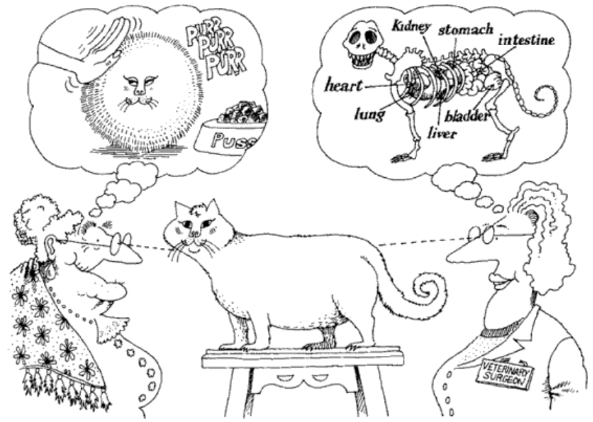
\includegraphics[width=0.45\textwidth]{abstraction.png}
        \end{center}
        \attribution{G. Booch, <<Object-oriented analysis and design>>}
    \end{frame}

    \begin{frame}
        \frametitle{Инкапсуляция}
        \textbf{Инкапсуляция} разделяет интерфейс (\textbf{контракты}) абстракции и её реализацию

        \vskip 1cm
        \begin{center}
            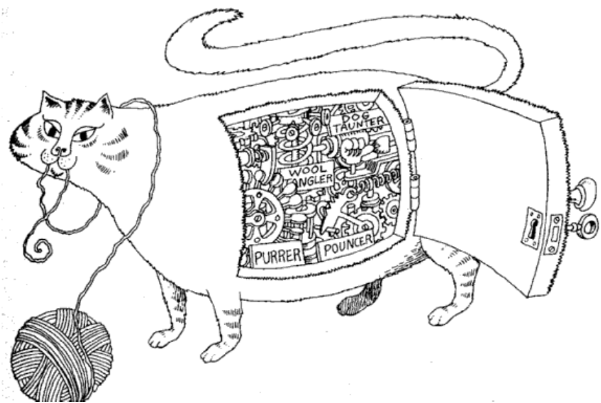
\includegraphics[width=0.45\textwidth]{incapsulation.png}
        \end{center}
        \attribution{G. Booch, <<Object-oriented analysis and design>>}
    \end{frame}

    \begin{frame}
        \frametitle{Инвариант объекта}
        Инкапсуляция защищает \textbf{инварианты} абстракции
        
        \textbf{Инвариант} --- набор условий на состояние объекта, которые выполняются всё время его жизни

        Например:
        \begin{itemize}
            \item Поле size списка должно содержать число, равное количеству элементов списка
            \item Поле next элемента списка, на который указывает поле prev текущего элемента, должно быть текущим элементом
            \item Баланс на счету мобильника больше нуля или нельзя звонить
        \end{itemize}

        Инвариант может нарушаться внутри метода, но восстанавливаться при его окончании

        \textbf{Объект сам отвечает за поддержание своих инвариантов}
    \end{frame}

    \begin{frame}
        \frametitle{Класс}
        \begin{itemize}
            \item \textbf{Класс} --- тип объекта (определяет поля и методы, которые могут быть у объекта)
            \item Бывают не во всех объектно-ориентированных языках 
            \item \textbf{Поля} --- собственно, состояние объекта
            \item \textbf{Поля класса} --- общее состояние ВСЕХ объектов данного класса
            \item \textbf{Методы} --- поведение объекта
            \item \textbf{Методы класса} --- поведение, не зависящее от состояния конкретного объекта (одинаковое для всех объектов данного класса)
        \end{itemize}
    \end{frame}

    \begin{frame}
        \frametitle{Наследование}
        \framesubtitle{Генерализация}
        \begin{columns}
            \begin{column}{0.75\textwidth}
                \begin{itemize}
                    \item \textbf{Генерализация} --- отношение между классами, связывающее более общее понятие и более конкретное
                    \begin{itemize}
                        \item Например, всякий студент --- человек (надеюсь)
                        \item Поэтому у каждого студента есть имя и фамилия, поскольку они есть у человека
                        \item То же с поведением, более частное понятие <<наследует>> поведение более общего
                    \end{itemize}
                \end{itemize}
            \end{column}
            \begin{column}{0.25\textwidth}
                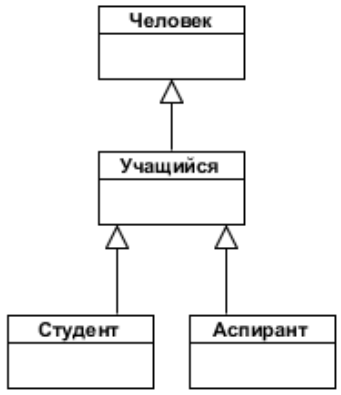
\includegraphics[width=\textwidth]{inheritance.png}
            \end{column}
        \end{columns}
    \end{frame}

    \begin{frame}
        \frametitle{Наследование}
        \framesubtitle{Cабтайпинг}
        \begin{itemize}
            \item Объект класса-потомка \textbf{является (is-a)} одновременно объектом класса предка
            \item И может быть использован везде, где может быть использован предок
            \item Отношение <<является>> и называется сабтайпингом (subtype polymorphism)
            \item Бывает наследование без сабтайпинга (например, в C++), бывает сабтайпинг  без наследования (например, в Паскале)
        \end{itemize}
    \end{frame}

    \begin{frame}[fragile]
        \frametitle{Типы времени компиляции и времени выполнения}
        \begin{itemize}
            \item Каждый объект на самом деле имеет много типов --- свой и всех своих предков
            \item Его <<настоящий>> тип --- \textbf{тип времени выполнения}
            \item Тип, по которому мы с ним работаем в конкретном месте программы --- \textbf{тип времени компиляции}
        \end{itemize}

        Пример:
        \begin{minted}{csharp}
Shape a = new Circle();
        \end{minted}
        Тип времени компиляции --- \textit{Shape}, следовательно у a можно вызывать только методы \textit{Shape}. 
        
        Тип времени выполнения --- \textit{Circle}.
    \end{frame}

    \begin{frame}[fragile]
        \frametitle{Полиморфизм}
        \begin{center}
            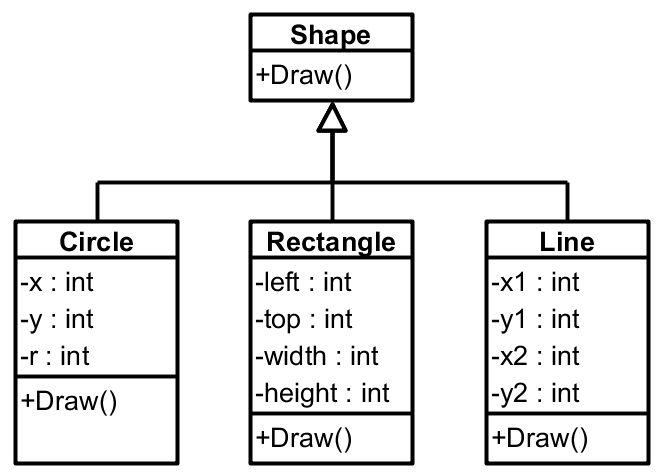
\includegraphics[width=0.4\textwidth]{polymorphism.png}
        \end{center}

        \begin{minted}{csharp}
List<Shape> shapes = new List { 
        new Circle(0, 0, 5), new Line(0, 0, 10, 10) };

foreach (var shape in shapes) 
{
    shape.Draw();
}
        \end{minted}
    \end{frame}

    \begin{frame}
        \frametitle{Абстрактные классы}
        \begin{itemize}
            \item Иногда у предка нет разумного поведения по умолчанию
            \begin{itemize}
                \item Например, что такое \textit{Draw} для просто \textit{Shape}?
            \end{itemize}
            \item Такие методы не реализуются, а остаются \textbf{абстрактными}
            \item Если у класса есть хоть один абстрактный метод, он не может порождать объекты
            \begin{itemize}
                \item То есть сам класс является абстрактным
            \end{itemize}
            \item \textbf{Интерфейс} --- класс, у которого все методы абстрактные
            \begin{itemize}
                \item Например, \textit{Shape} мог бы быть интерфейсом
            \end{itemize}
            \item На самом деле, интерфейс --- это контракт класса
        \end{itemize}
    \end{frame}
    
    \section{ООП в C\#}

    \begin{frame}[fragile]
        \frametitle{Ссылочные типы и типы-значения}
        \begin{center}
            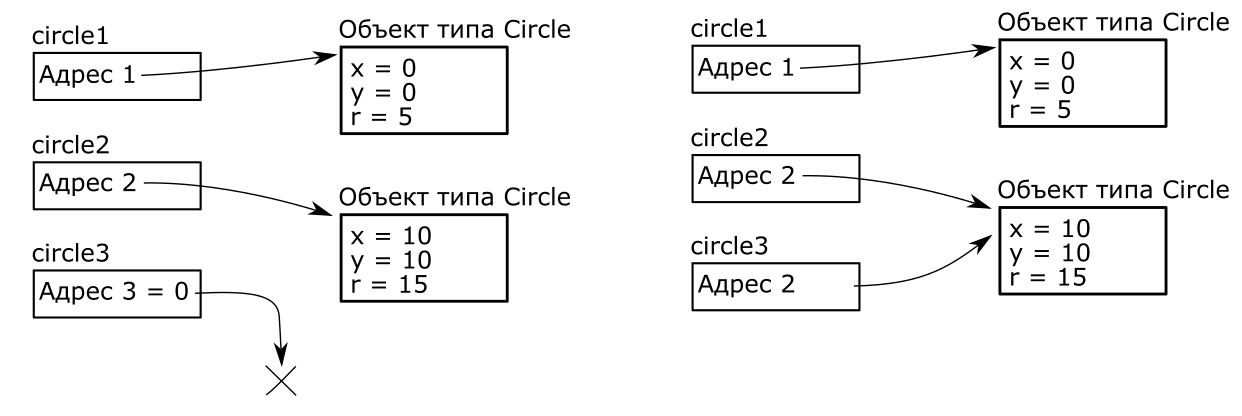
\includegraphics[width=\textwidth]{referenceTypes.png}
        \end{center}
        \begin{minted}{csharp}
var circle1 = new Circle(0, 0, 5);
var circle2 = new Circle(10, 10, 15);
var circle3 = null;

circle3 = circle2;
        \end{minted}
    \end{frame}

    \begin{frame}
        \frametitle{Ссылочные типы и типы-значения в C\#}
        Ссылочные типы:
        \begin{itemize}
            \item Пользовательские классы
            \item Строки
            \item Массивы
            \item Исключения
            \item Делегаты
        \end{itemize}

        Типы-значения:
        \begin{itemize}
            \item Примитивные типы
            \item Перечисления
            \item Структуры
        \end{itemize}
    \end{frame}
    
        \begin{frame}[fragile]
        \frametitle{Пример}
        \begin{minted}{csharp}
static void Add(string s1, string s2, string s3)
{
    s3 = s1 + s2;
}

private static void Main(string[] args)
{
    string s1 = "a";
    string s2 = "b";
    string s3 = "c";
    Add(s1, s2, s3);
}
        \end{minted}
    \end{frame}

    \begin{frame}[fragile]
        \frametitle{Передача параметров по ссылке}
        \begin{minted}{csharp}
static void Add(string s1, string s2, ref string s3)
{
    s3 = s1 + s2;
}

private static void Main(string[] args)
{
    string s1 = "a";
    string s2 = "b";
    string s3 = "c";
    Add(s1, s2, ref s3);
}
        \end{minted}
    \end{frame}

    \begin{frame}[fragile]
        \frametitle{Out-параметры}
        \begin{minted}{csharp}
static void Add(string s1, string s2, out string s3)
{
    s3 = s1 + s2;
}

private static void Main(string[] args)
{
    string s1 = "a";
    string s2 = "b";
    Add(s1, s2, out string s3);
    Console.WriteLine(s3);
}
        \end{minted}
    \end{frame}

    \begin{frame}[fragile]
        \frametitle{На самом деле, это не нужно}
        \begin{minted}{csharp}
static string Add(string s1, string s2)
{
    return s1 + s2;
}

private static void Main(string[] args)
{
    string s1 = "a";
    string s2 = "b";
    string s3 = Add(s1, s2);
    Console.WriteLine(s3);
}
        \end{minted}
        C\# умеет возвращать пары, тройки и т.д.
    \end{frame}

    \begin{frame}[fragile]
        \frametitle{Конструкторы}
        \begin{minted}{csharp}
class Circle
{
    public Circle(int x, int y, int r)
    {
        this.x = x;
        this.y = y;
        this.r = r;
    }

    private int x;
    private int y;
    private int r;
}
        \end{minted}
    \end{frame}

    \begin{frame}[fragile]
        \frametitle{Перегрузка конструкторов, chaining}
        \begin{small}
            \begin{minted}{csharp}
class Circle
{
    public Circle(int x, int y, int r)
    {
        this.x = x;
        this.y = y;
        this.r = r;
    }

    public Circle(int r)
        : this(0, 0, r)
    {
    }

    private int x;
    private int y;
    private int r;
}
            \end{minted}
        \end{small}
    \end{frame}

    \begin{frame}[fragile]
        \frametitle{Наследование (1)}
        \begin{minted}{csharp}
class Shape
{
    public Shape()
    {
    }

    public Shape(int x, int y)
    {
        this.x = x;
        this.y = y;
    }

    protected int x;
    protected int y;
}
        \end{minted}
    \end{frame}

    \begin{frame}[fragile]
        \frametitle{Наследование (2)}
        \begin{minted}{csharp}
class Circle : Shape
{
    Circle(int x, int y, int r)
    {
        this.x = x;
        this.y = y;
        this.r = r;
    }

    Circle(int r)
        : base(0, 0)
    {
    }

    private int r;
}
        \end{minted}
    \end{frame}

    \begin{frame}[fragile]
        \frametitle{Интерфейсы}
        \begin{minted}{csharp}
interface IDrawable
{
    void Draw();
}
        \end{minted}
    \end{frame}

    \begin{frame}[fragile]
        \frametitle{Реализация интерфейса}
        \begin{minted}{csharp}
class Shape : IDrawable
{
    public void Draw()
    {
        Console.Write("Drawing Shape");
    }

    protected int x;
    protected int y;
}
        \end{minted}
    \end{frame}

    \begin{frame}[fragile]
        \frametitle{Явная реализация интерфейса}
        \begin{minted}{csharp}
class Shape : IDrawable
{
    void IDrawable.Draw()
    {
        Console.Write("Drawing Shape");
    }

    protected int x;
    protected int y;
}
        \end{minted}
    \end{frame}

    \begin{frame}[fragile]
        \frametitle{Зачем}
        \begin{footnotesize}
            \begin{minted}{csharp}
interface IDrawable {
    void Draw();
}

interface IMySpecialDrawable {
    void Draw();
}

class Shape : IDrawable, IMySpecialDrawable
{
    void IDrawable.Draw()
        => Console.Write("Drawing Shape");

    void IMySpecialDrawable.Draw()
        => Console.Write("Drawing Shape, but completely unrelated to IDrawable");

    protected int x;
    protected int y;
}
            \end{minted}
        \end{footnotesize}
    \end{frame}

    \begin{frame}[fragile]
        \frametitle{И вот что будет}
        \begin{minted}{csharp}
var shape = new Shape();
shape.Draw();  // Ошибка компиляции
((IDrawable)shape).Draw();  // Drawing Shape
((IMySpecialDrawable)shape).Draw();  // Drawing Shape, but...
        \end{minted}
    \end{frame}

    \begin{frame}[fragile]
        \frametitle{Абстрактные классы}
        \begin{minted}{csharp}
abstract class Shape
{
    public Shape() 
    {
    }

    public abstract void Draw();

    protected int x;
    protected int y;
}
        \end{minted}
    \end{frame}

    \begin{frame}[fragile]
        \frametitle{Виртуальные методы (1)}
        \begin{minted}{csharp}
class Shape
{
    public virtual void Draw()
    {
        Console.WriteLine(
                $"Drawing Shape with coords ({x}, {y})");
    }

    protected int x;
    protected int y;
}
        \end{minted}
    \end{frame}

    \begin{frame}[fragile]
        \frametitle{Виртуальные методы (2)}
        \begin{minted}{csharp}
class Circle : Shape
{
    public Circle(int x, int y, int r)
    {
        this.x = x;
        this.y = y;
        this.r = r;
    }

    public override void Draw()
    {
        Console.WriteLine($"Drawing Circle with radius {r}");
    }

    private int r;
}
        \end{minted}
    \end{frame}

    \begin{frame}[fragile]
        \frametitle{Виртуальные методы (3)}
        \begin{footnotesize}
            \begin{minted}{csharp}
class Rectangle : Shape
{
    public Rectangle(int x, int y, int width, int height)
    {
        this.x = x;
        this.y = y;
        this.width = width;
        this.height = height;
    }
    public override void Draw()
    {
        base.Draw();
        Console.WriteLine(
            $"Drawing Rectangle with width={width} and height={height}");
    }
    protected int width;
    protected int height;
}
            \end{minted}
        \end{footnotesize}
    \end{frame}

    \begin{frame}[fragile]
        \frametitle{Виртуальные методы (4)}
        \begin{minted}{csharp}
private static void Main(string[] args)
{
    var circle = new Circle(0, 0, 10);
    var rectangle = new Rectangle(0, 0, 10, 10);
    var list = new System.Collections.Generic.List<Shape>();
    list.Add(circle);
    list.Add(rectangle);
    foreach (var shape in list)
    {
        shape.Draw();
    }
}
        \end{minted}
    \end{frame}

    \begin{frame}[fragile]
        \frametitle{Абстрактные методы}
        \begin{minted}{csharp}
abstract class Shape
{
    public abstract void Draw();

    protected int x;
    protected int y;
}
        \end{minted}
\end{frame}

    \begin{frame}[fragile]
        \frametitle{Перевведение методов, new (1)}
        \begin{minted}{csharp}
class Shape
{
    public virtual void Draw()
    {
        Console.WriteLine(
                $"Drawing Shape with coords ({x}, {y})");
    }

    protected int x;
    protected int y;
}
        \end{minted}
    \end{frame}

    \begin{frame}[fragile]
        \frametitle{Перевведение методов, new (2)}
        \begin{small}
            \begin{minted}{csharp}
class Circle : Shape
{
    public Circle(int x, int y, int r)
    {
        this.x = x;
        this.y = y;
        this.r = r;
    }

    public new void Draw()
    {
        Console.WriteLine($"Drawing Circle with radius {r}");
    }

    private int r;
}
            \end{minted}
        \end{small}
    \end{frame}

    \begin{frame}[fragile]
        \frametitle{Перевведение методов, new (3)}
        \begin{minted}{csharp}
Circle circle1 = new Circle(10, 10, 3);
Shape circle2 = new Circle(10, 10, 3);
var circle3 = new Circle(10, 10, 3);

circle1.Draw();
circle2.Draw();
circle3.Draw();
        \end{minted}
        \vspace{1cm}
        Лучше про это забыть и никогда не пользоваться, хотя на собеседованиях спрашивают
    \end{frame}

    \begin{frame}
        \frametitle{Модификаторы видимости}
        \begin{itemize}
            \item \mintinline{csharp}|public| --- применяется к типам и членам, доступ без ограничений
            \item \mintinline{csharp}|protected| --- применяется только к членам, доступ в типе и потомках
            \item \mintinline{csharp}|internal| --- применяется к типам и членам, доступ внутри сборки
            \item \mintinline{csharp}|protected internal| --- применяется к типам и членам, доступ внутри сборки \textbf{или} в потомках
            \item \mintinline{csharp}|private| --- применяется к типам и членам, доступ только внутри типа
            \item По умолчанию для типов \mintinline{csharp}|internal|, для членов --- \mintinline{csharp}|private|
        \end{itemize}
    \end{frame}

    \begin{frame}
        \frametitle{Другие модификаторы}
        \begin{itemize}
            \item \mintinline{csharp}|partial| --- <<частичный>> класс, декларирует, что определение класса разбито на несколько файлов
            \begin{itemize}
                \item Для интеграции сгенерированного и рукописного кода, не используйте без нужды
            \end{itemize}
            \item \mintinline{csharp}|sealed| --- запрещение наследования от класса
            \item \mintinline{csharp}|static| --- не может быть инстанцирован, может содержать только \mintinline{csharp}|static|-методы
        \end{itemize}
    \end{frame}

    \begin{frame}[fragile]
        \frametitle{Вложенные классы}
        \begin{scriptsize}
            \begin{minted}{csharp}
class Circle
{
    private readonly Point pos;
    private readonly int r;

    private class Point
    {
        public int x;
        public int y;
    }

    public Circle(int x, int y, int r)
    {
        pos = new Point {x = 10, y = 10};
        this.r = r;
    }

    public void Draw() =>
        Console.WriteLine($"({pos.x}, {pos.y}), radius {r}");
}
            \end{minted}
        \end{scriptsize}
    \end{frame}

    \begin{frame}[fragile]
        \frametitle{Преобразования типов}
        \begin{minted}{csharp}
Shape shape = new Circle();
Circle circle = (Circle)shape;

Circle circle = shape as Circle;

if (shape is Circle)
{
    Circle circle = (Circle)shape;
}

if (shape is Circle circle)
{
}
        \end{minted}
    \end{frame}

    \begin{frame}[fragile]
        \frametitle{Сопоставление шаблонов}
        \begin{small}
            \begin{minted}{csharp}
switch (shape)
{
    case Circle c:
        WriteLine($"circle with radius {c.Radius}");
        break;
    case Rectangle s when (s.Length == s.Height):
        WriteLine($"{s.Length} x {s.Height} square");
        break;
    case Rectangle r:
        WriteLine($"{r.Length} x {r.Height} rectangle");
        break;
    default:
        WriteLine("<unknown shape>");
        break;
    case null:
        throw new ArgumentNullException(nameof(shape));
}
            \end{minted}
        \end{small}
\end{frame}

\begin{frame}
    \frametitle{Иерархия основных классов}
    \begin{tiny}
        \begin{forest}
            for tree={rectangle,draw,l sep=1cm,s sep=5mm,edge=open triangle 60-}
            [Object
                [ValueType
                    [Enum]
                    [Элементарные типы]
                    [Пользовательские структуры]
                ]
                [Array]
                [Delegate]
                [Exception]
                [Пользовательские классы]
                [...]
            ]
        \end{forest}
    \end{tiny}
\end{frame}

\begin{frame}
    \frametitle{Методы System.Object}
    \begin{itemize}
        \item Equals --- виртуальный
        \item GetHashCode --- виртуальный
        \item ToString --- виртуальный
        \item GetType --- невиртуальный
        \item MemberwiseClone --- невиртуальный защищённый
        \begin{itemize}
            \item Создаёт объект, не вызывая конструктор
        \end{itemize}
        \item Finalize --- виртуальный защищённый
    \end{itemize}
\end{frame}

\begin{frame}[fragile]
    \frametitle{Объекты в памяти}
    \begin{columns}
        \begin{column}{0.4\textwidth}
            \begin{minted}{csharp}
void Example() 
{
    Employee e = 
        new Manager();
    e.GenProgressReport();
}
            \end{minted}
        \end{column}
        \begin{column}{0.6\textwidth}
            \begin{center}
                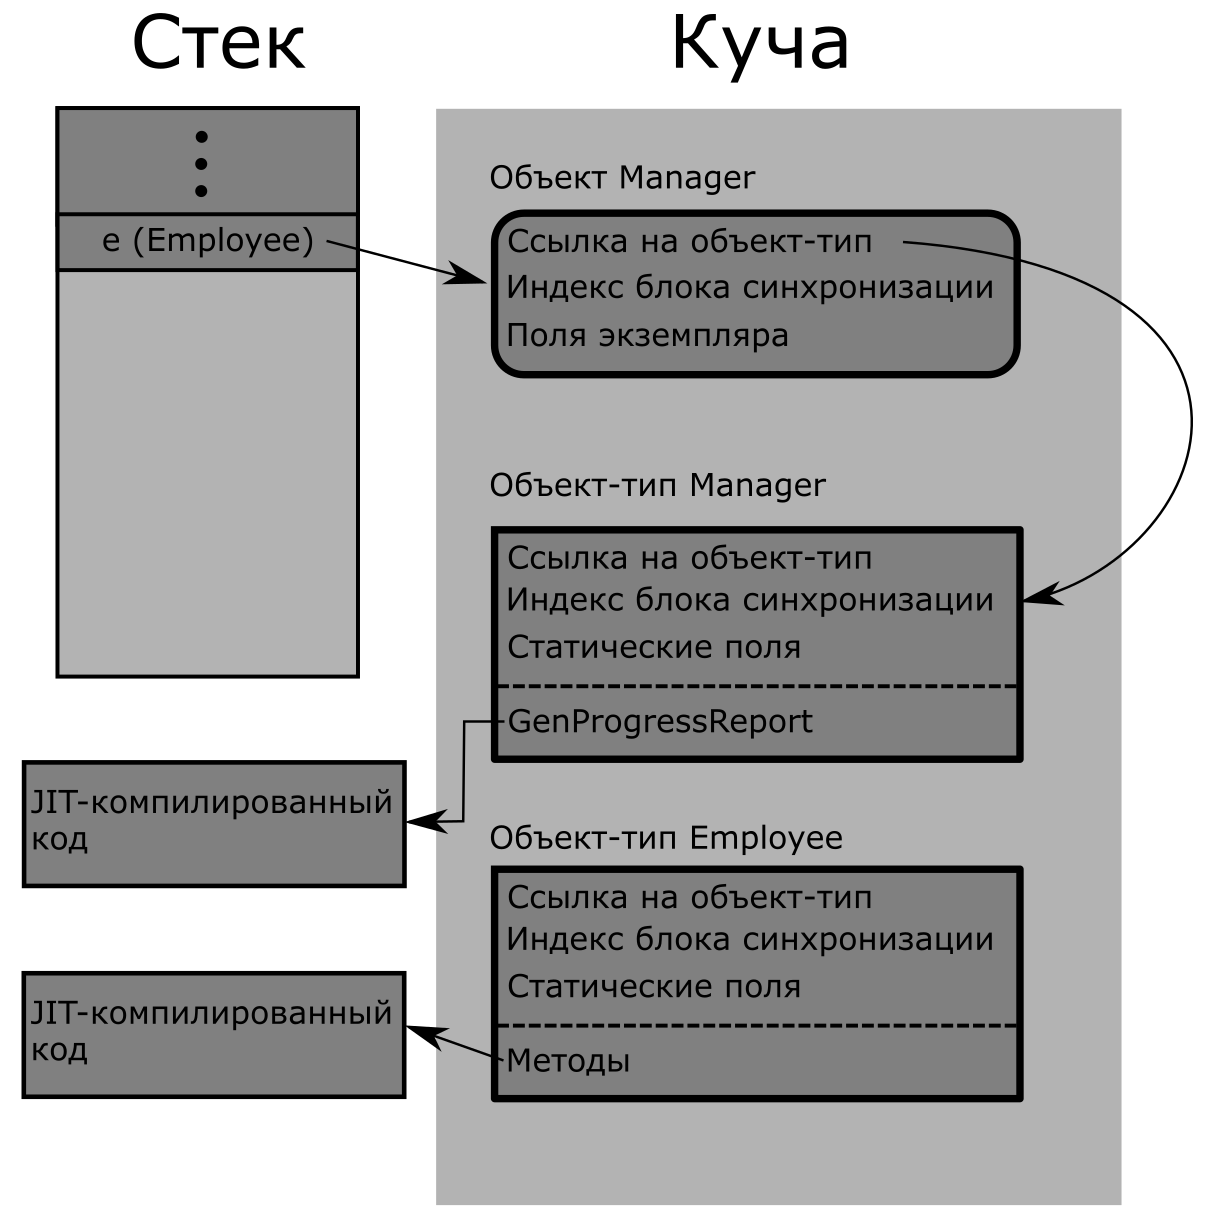
\includegraphics[width=0.8\textwidth]{objectInMemory.png}
            \end{center}
        \end{column}
    \end{columns}
\end{frame}

\end{document}